%%%%%%%%%%%%%%%%%%%%%%%%%%%%%%%%%%%%%%%%%}}
% Beamer Presentation - LaTeX Template
% Version 2.0 (March 8, 2022)
% Original Template: https://www.LaTeXTemplates.com
% Author: Vel (vel@latextemplates.com)
% License: CC BY-NC-SA 4.0

% Este modelo de apresentação foi 
% criado a partir do modelo de Giovanni Spadaro.
% Disponível em: https://github.com/Giovo17/presentation-template-unict-lm-data
%
% Adaptado por Lucas Amaral Taylor para criar uma versão especial 
% para os alunos de Matemática e Estatística da USP (IME-USP).
% Disponível em: https://github.com/lucasamtaylor01/IME-template
%%%%%%%%%%%%%%%%%%%%%%%%%%%%%%%%%%%%%%%%%

%----------------------------------------------------------------------------------------
% CLASSE DO DOCUMENTO E CONFIGURAÇÕES BÁSICAS
%----------------------------------------------------------------------------------------
\documentclass[aspectratio=169]{beamer}
\graphicspath{{img/}}         % 指定图像文件的存储路径为 img/ 文件夹

%----------------------------------------------------------------------------------------
% PACOTES NECESSÁRIOS
%----------------------------------------------------------------------------------------
\usepackage{
    booktabs,     % 优化表格的线条样式
    palatino,     % 设置主字体为 Palatino
    ctex,         % 中文核心包
    subcaption    % 支持子图(subfigures)
}
\usepackage[default]{opensans}              % 设置辅助字体为 Open Sans
\usepackage{graphicx}
\usepackage{caption}
%----------------------------------------------------------------------------------------
%	PACOTES E CONFIGURAÇÕES PARA CÓDIGO
%----------------------------------------------------------------------------------------
% Pacotes necessários para formatação de código
\usepackage[utf8]{inputenc}
\usepackage{listings}
\usepackage{xcolor}

% Cores para syntax highlighting (VSCode Light Theme)
\definecolor{vscBackground}{RGB}{255,255,255}    % Fundo branco
\definecolor{vscKeyword}{RGB}{175,0,219}         % Roxo para palavras-chave
\definecolor{vscString}{RGB}{163,21,21}          % Vermelho para strings
\definecolor{vscComment}{RGB}{0,128,0}           % Verde para comentários
\definecolor{vscFunction}{RGB}{121,94,38}        % Marrom para funções
\definecolor{vscNumber}{RGB}{9,134,88}           % Verde escuro para números
\definecolor{vscOperator}{RGB}{175,0,219}        % Roxo para operadores
\definecolor{vscText}{RGB}{0,0,0}                % Texto preto
\definecolor{vscLineNr}{RGB}{128,128,128}        % Cinza para números de linha

% Configuração geral do listings para UTF-8
\lstset{
    inputencoding=utf8,
    extendedchars=true,
    literate=%
        {á}{{\'a}}1 {é}{{\'e}}1 {í}{{\'i}}1 {ó}{{\'o}}1 {ú}{{\'u}}1
        {Á}{{\'A}}1 {É}{{\'E}}1 {Í}{{\'I}}1 {Ó}{{\'O}}1 {Ú}{{\'U}}1
        {à}{{\`a}}1 {è}{{\`e}}1 {ì}{{\`i}}1 {ò}{{\`o}}1 {ù}{{\`u}}1
        {À}{{\`A}}1 {È}{{\'E}}1 {Ì}{{\`I}}1 {Ò}{{\`O}}1 {Ù}{{\`U}}1
        {ã}{{\~a}}1 {ẽ}{{\~e}}1 {ĩ}{{\~i}}1 {õ}{{\~o}}1 {ũ}{{\~u}}1
        {Ã}{{\~A}}1 {Ẽ}{{\~E}}1 {Ĩ}{{\~I}}1 {Õ}{{\~O}}1 {Ũ}{{\~U}}1
        {â}{{\^a}}1 {ê}{{\^e}}1 {î}{{\^i}}1 {ô}{{\^o}}1 {û}{{\^u}}1
        {Â}{{\^A}}1 {Ê}{{\^E}}1 {Î}{{\^I}}1 {Ô}{{\^O}}1 {Û}{{\^U}}1
        {ç}{{\c c}}1 {Ç}{{\c C}}1
        {º}{{\textordmasculine}}1
        {ª}{{\textordfeminine}}1
}

% Configurações base comum para todas as linguagens
\lstdefinestyle{baseStyle}{
    backgroundcolor=\color{vscBackground},
    basicstyle=\ttfamily\small\color{vscText},
    breakatwhitespace=false,
    breaklines=true,
    captionpos=b,
    keepspaces=true,
    numbers=left,
    numbersep=5pt,
    showspaces=false,
    showstringspaces=false,
    showtabs=false,
    tabsize=4,
    frame=single,
    framerule=0.8pt,
    rulecolor=\color{gray!20},
    numberstyle=\tiny\color{vscLineNr},
    keywordstyle=\color{vscKeyword},
    commentstyle=\color{vscComment}\itshape,
    stringstyle=\color{vscString},
    emphstyle=\color{vscFunction},
    columns=flexible,
    basewidth={0.5em,0.45em},
    inputencoding=utf8,
    extendedchars=true
}

%----------------------------------------------------------------------------------------
% Python
%----------------------------------------------------------------------------------------
\lstdefinestyle{pythonStyle}{
    style=baseStyle,
    language=Python,
    morekeywords={self,None,True,False,import,from,as,def,class,return,yield,
                  for,while,if,else,elif,try,except,finally,with,lambda,
                  async,await,break,continue,global,nonlocal,pass,raise},
    morekeywords=[2]{print,len,range,type,int,str,float,list,dict,set,
                     tuple,max,min,sum,sorted,enumerate,zip,map,filter,
                     any,all,abs,round,pow,divmod},
    keywordstyle=[2]\color{vscFunction},
    sensitive=true
}

\lstnewenvironment{python}[1][]{\lstset{style=pythonStyle, #1}}{}
\newcommand{\pyinline}[1]{\lstinline[style=pythonStyle]!#1!}
\newcommand{\inputpython}[2][]{\lstinputlisting[style=pythonStyle,#1]{#2}}

%----------------------------------------------------------------------------------------
% C Language
%----------------------------------------------------------------------------------------
\lstdefinestyle{cStyle}{
    style=baseStyle,
    language=C,
    morekeywords={include,define,void,int,char,float,double,long,unsigned,
                  struct,union,enum,typedef,const,static,extern,register,
                  auto,volatile,sizeof,return,if,else,for,while,do,switch,
                  case,break,continue,default,goto},
    morekeywords=[2]{printf,scanf,malloc,free,calloc,realloc,fopen,fclose,
                     fprintf,fscanf,strcpy,strlen,strcat},
    keywordstyle=[2]\color{vscFunction},
    sensitive=true
}

\lstnewenvironment{clang}[1][]{\lstset{style=cStyle, #1}}{}
\newcommand{\clinline}[1]{\lstinline[style=cStyle]!#1!}
\newcommand{\inputclang}[2][]{\lstinputlisting[style=cStyle,#1]{#2}}

%----------------------------------------------------------------------------------------
% C++
%----------------------------------------------------------------------------------------
\lstdefinestyle{cppStyle}{
    style=baseStyle,
    language=C++,
    morekeywords={class,private,protected,public,template,typename,namespace,
                  using,new,delete,this,friend,virtual,override,final,explicit,
                  mutable,constexpr,nullptr,noexcept,static_cast,dynamic_cast,
                  const_cast},
    morekeywords=[2]{cout,cin,endl,vector,string,map,set,queue,stack,pair,
                     begin,end,push_back,pop_back,emplace_back,size,empty},
    keywordstyle=[2]\color{vscFunction},
    sensitive=true
}

\lstnewenvironment{cpp}[1][]{\lstset{style=cppStyle, #1}}{}
\newcommand{\cppinline}[1]{\lstinline[style=cppStyle]!#1!}
\newcommand{\inputcpp}[2][]{\lstinputlisting[style=cppStyle,#1]{#2}}

%----------------------------------------------------------------------------------------
% R Language
%----------------------------------------------------------------------------------------
\lstdefinestyle{rStyle}{
    style=baseStyle,
    language=R,
    morekeywords={if,else,repeat,while,function,for,in,next,break,TRUE,FALSE,
                  NULL,Inf,NaN,NA,NA_integer_,NA_real_,NA_complex_,NA_character_},
    morekeywords=[2]{library,require,attach,detach,source,setwd,options,
                     data.frame,read.csv,write.csv,list,matrix,array},
    keywordstyle=[2]\color{vscFunction},
    sensitive=true
}

\lstnewenvironment{rlang}[1][]{\lstset{style=rStyle, #1}}{}
\newcommand{\rlinline}[1]{\lstinline[style=rStyle]!#1!}
\newcommand{\inputrlang}[2][]{\lstinputlisting[style=rStyle,#1]{#2}}

%----------------------------------------------------------------------------------------
% Java
%----------------------------------------------------------------------------------------
\lstdefinestyle{javaStyle}{
    style=baseStyle,
    language=Java,
    morekeywords={abstract,assert,boolean,break,byte,case,catch,char,class,
                  const,continue,default,do,double,else,enum,extends,final,
                  finally,float,for,if,implements,import,instanceof,int,
                  interface,long,native,new,package,private,protected,public,
                  return,short,static,strictfp,super,switch,synchronized,this,
                  throw,throws,transient,try,void,volatile,while},
    morekeywords=[2]{String,System,out,println,printStackTrace,ArrayList,
                     HashMap,Arrays,List,Map,Set,Exception,RuntimeException},
    keywordstyle=[2]\color{vscFunction},
    sensitive=true
}

\lstnewenvironment{java}[1][]{\lstset{style=javaStyle, #1}}{}
\newcommand{\javainline}[1]{\lstinline[style=javaStyle]!#1!}
\newcommand{\inputjava}[2][]{\lstinputlisting[style=javaStyle,#1]{#2}}                   % 加载代码高亮配置
\setCJKmainfont{TW-Kai}

%----------------------------------------------------------------------------------------
% CONFIGURAÇÃO DO TEMA
%----------------------------------------------------------------------------------------
% Tema Base
\usetheme{Madrid}
\usecolortheme{default}
\useinnertheme{circles}                      % 内部主题,使用圆形样式
\useoutertheme{miniframes}                   % 外部主题,显示导航条中的小帧
\setbeamertemplate{navigation symbols}{}     % 移除导航符号(如箭头等)

% 自定义两种颜色
\definecolor{primaryColor}{RGB}{20,45,105}   % primaryColor:深蓝色
\definecolor{secondaryColor}{RGB}{0,100,160} % secondaryColor:中蓝色

% 设置 Beamer 的颜色主题
\setbeamercolor{structure}{fg=primaryColor}
\setbeamercolor{palette primary}{bg=primaryColor, fg=white}
\setbeamercolor{palette secondary}{bg=secondaryColor, fg=white}
\setbeamercolor{title}{bg=primaryColor, fg=white}

% 头部和底部颜色
\setbeamercolor{headline}{bg=secondaryColor, fg=white}
\setbeamercolor{section in head/foot}{bg=primaryColor, fg=white}
\setbeamercolor{subsection in head/foot}{bg=secondaryColor, fg=white}
\setbeamercolor{author in head/foot}{bg=primaryColor, fg=white}
\setbeamercolor{title in head/foot}{bg=secondaryColor, fg=white}
\setbeamercolor{date in head/foot}{bg=primaryColor, fg=white}
\setbeamercolor{page number in head/foot}{bg=primaryColor, fg=white}

%----------------------------------------------------------------------------------------
% 引用管理
%----------------------------------------------------------------------------------------
\usepackage[style=alphabetic,backend=biber]{biblatex}   % 使用 biblatex 包管理参考文献,style=alphabetic:引用风格为字母编号,backend=biber:使用 Biber 作为后端
\addbibresource{bibliografia.bib}                       % bibliografia.bib:引用的 .bib 文件

%----------------------------------------------------------------------------------------
% 演示文稿信息
%----------------------------------------------------------------------------------------
\title{基于GRPO的坐标序列预测}
\subtitle{自然语言处理课程项目}
\author{王阳 \and 周齐圣 \and 刘涵 \and 郑思华}
\institute{计算机科学与技术学院}
\date{2025年6月}

%----------------------------------------------------------------------------------------
% INÍCIO DO DOCUMENTO
%----------------------------------------------------------------------------------------
\begin{document}

% 标题页
\begin{frame}
    \begin{figure}
        % \includegraphics[width=0.45\linewidth]{img/logo_IME.png}
    \end{figure}
    \titlepage
\end{frame}

% 目录页
\begin{frame}
    \frametitle{目录}
    \tableofcontents
\end{frame}

% 导入每个section
\section{项目介绍}
\section{GRPO算法讲解}
\section{实验框架与代码展示}
\section{实验结果}
\section{创新点}

\begin{frame}{创新亮点总览}
    \begin{columns}[t]
        \begin{column}{0.48\textwidth}
            \textbf{算法创新}
            \begin{itemize}
                \item 首次将GRPO应用于坐标预测
                \item 设计特定的奖励函数体系
                \item 优化的组采样策略
            \end{itemize}
            \vspace{0.3cm}
            \textbf{工程实现}
            \begin{itemize}
                \item 高效的数据生成框架
                \item 模块化的实验系统
                \item 创新的评估指标
            \end{itemize}
        \end{column}
        \begin{column}{0.48\textwidth}
            \textbf{应用创新}
            \begin{itemize}
                \item Chain-of-Thought推理
                \item 动态批次优化
                \item 分布式训练支持
            \end{itemize}
            \vspace{0.3cm}
            \textbf{实验突破}
            \begin{itemize}
                \item 优异的泛化性能
                \item 显著的效率提升
                \item 稳定的训练过程
            \end{itemize}
        \end{column}
    \end{columns}
\end{frame}

\begin{frame}{核心技术指标}
    \begin{block}{性能提升}
        \begin{itemize}
            \item 训练速度提升40\%(相比传统PPO)
            \item 内存占用降低35\%
            \item 预测准确率达90\%(分布内)
            \item 泛化性能提升25\%(分布外)
        \end{itemize}
    \end{block}
    
    \begin{alertblock}{关键技术亮点}
        \begin{enumerate}
            \item \textbf{双重奖励机制}:结合准确性奖励与格式奖励
            \item \textbf{自适应采样}:动态调整组采样数量
            \item \textbf{高效推理}:优化的Chain-of-Thought设计
        \end{enumerate}
    \end{alertblock}
\end{frame}

\begin{frame}{技术创新细节}
    \begin{block}{奖励函数设计}
        \begin{itemize}
            \item 准确性奖励:基于MSE的预测评估
            \item 格式奖励:评估推理过程完整性
            \item 权重比例:5:1(准确性vs格式)
        \end{itemize}
    \end{block}
    
    \begin{block}{组采样优化}
        \begin{itemize}
            \item 动态批次大小调整
            \item 自适应的组采样数量(4-8个)
            \item 智能的显存管理机制
        \end{itemize}
    \end{block}
    
    \begin{block}{推理框架改进}
        \begin{itemize}
            \item 结构化的分析步骤设计
            \item 优化的Chain-of-Thought模板
            \item 高效的数据流水线
        \end{itemize}
    \end{block}
\end{frame}

\begin{frame}{未来展望}
    \begin{block}{技术拓展}
        \begin{itemize}
            \item 扩展到更复杂的运动模式预测
            \item 探索多维坐标序列的预测
            \item 研究更高效的奖励计算方法
        \end{itemize}
    \end{block}
    
    \begin{block}{工程优化}
        \begin{itemize}
            \item 开发自动化的超参数优化
            \item 完善分布式训练框架
            \item 构建可视化评估工具
        \end{itemize}
    \end{block}
    
    \begin{alertblock}{应用价值}
        本项目的创新不仅限于坐标预测任务,其核心技术可推广到:
        \begin{itemize}
            \item 其他序列预测任务
            \item 大规模语言模型训练
            \item 通用强化学习应用
        \end{itemize}
    \end{alertblock}
\end{frame}  % 标题页和目录
% Seções são adicionadas para organizar sua apresentação em blocos discretos, todas as seções e subseções são automaticamente exibidas no índice como uma visão geral da apresentação, mas NÃO são exibidas como slides separados.

%----------------------------------------------------------------------------------------



% \begin{frame}{Uma imagem}
%    \begin{figure}[h]
%        \centering
%        \includegraphics[width=0.7\textwidth]{img/logo_IME.png}
%        \caption{Legenda da imagem}
%        \label{fig:label_da_imagem}
%    \end{figure}
% \end{frame}

% %----------------------------------------------------------------------------------------

% \begin{frame}{Duas imagens}
%    \begin{figure}
%        \centering
%        \begin{subfigure}[b]{0.45\textwidth}
%            \centering
%            \includegraphics[width=\textwidth]{img/logo_IME.png}
%            \caption{Legenda 1}
%            \label{fig:img1}
%        \end{subfigure}
%        \hfill
%        \begin{subfigure}[b]{0.45\textwidth}
%            \centering
%            \includegraphics[width=\textwidth]{img/logo_IME.png}
%            \caption{Legenda 2}
%            \label{fig:img2}
%        \end{subfigure}
%    \end{figure}
% \end{frame}

% %----------------------------------------------------------------------------------------
% \begin{frame}{Equações}
%     Equações de Navier-Stokes Forma expandida (3D):
%     \footnotesize
%         \begin{align*}
%             \rho\left(\frac{\partial u}{\partial t} + u\frac{\partial u}{\partial x} + v\frac{\partial u}{\partial y} + w\frac{\partial u}{\partial z}\right) &= -\frac{\partial p}{\partial x} + \mu\left(\frac{\partial^2 u}{\partial x^2} + \frac{\partial^2 u}{\partial y^2} + \frac{\partial^2 u}{\partial z^2}\right) + f_x \\[0.3cm]
%             \rho\left(\frac{\partial v}{\partial t} + u\frac{\partial v}{\partial x} + v\frac{\partial v}{\partial y} + w\frac{\partial v}{\partial z}\right) &= -\frac{\partial p}{\partial y} + \mu\left(\frac{\partial^2 v}{\partial x^2} + \frac{\partial^2 v}{\partial y^2} + \frac{\partial^2 v}{\partial z^2}\right) + f_y \\[0.3cm]
%             \rho\left(\frac{\partial w}{\partial t} + u\frac{\partial w}{\partial x} + v\frac{\partial w}{\partial y} + w\frac{\partial w}{\partial z}\right) &= -\frac{\partial p}{\partial z} + \mu\left(\frac{\partial^2 w}{\partial x^2} + \frac{\partial^2 w}{\partial y^2} + \frac{\partial^2 w}{\partial z^2}\right) + f_z
%         \end{align*}
        
%     onde $\mathbf{v} = (u,v,w)$ é o campo de velocidade, $p$ é a pressão, $\rho$ é a densidade, $\mu$ é a viscosidade dinâmica e $\mathbf{f}$ representa forças externas.
% \end{frame}

\section{算法设计}

% GRPO算法框架
\begin{frame}{GRPO算法框架}
    \begin{columns}
        \column{0.5\textwidth}
        \begin{itemize}
            \item \textbf{核心创新}
            \begin{itemize}
                \item 无价值网络设计
                \item 生成式奖励处理
                \item 组采样机制
            \end{itemize}
        \end{itemize}
        \column{0.5\textwidth}
        \begin{figure}
            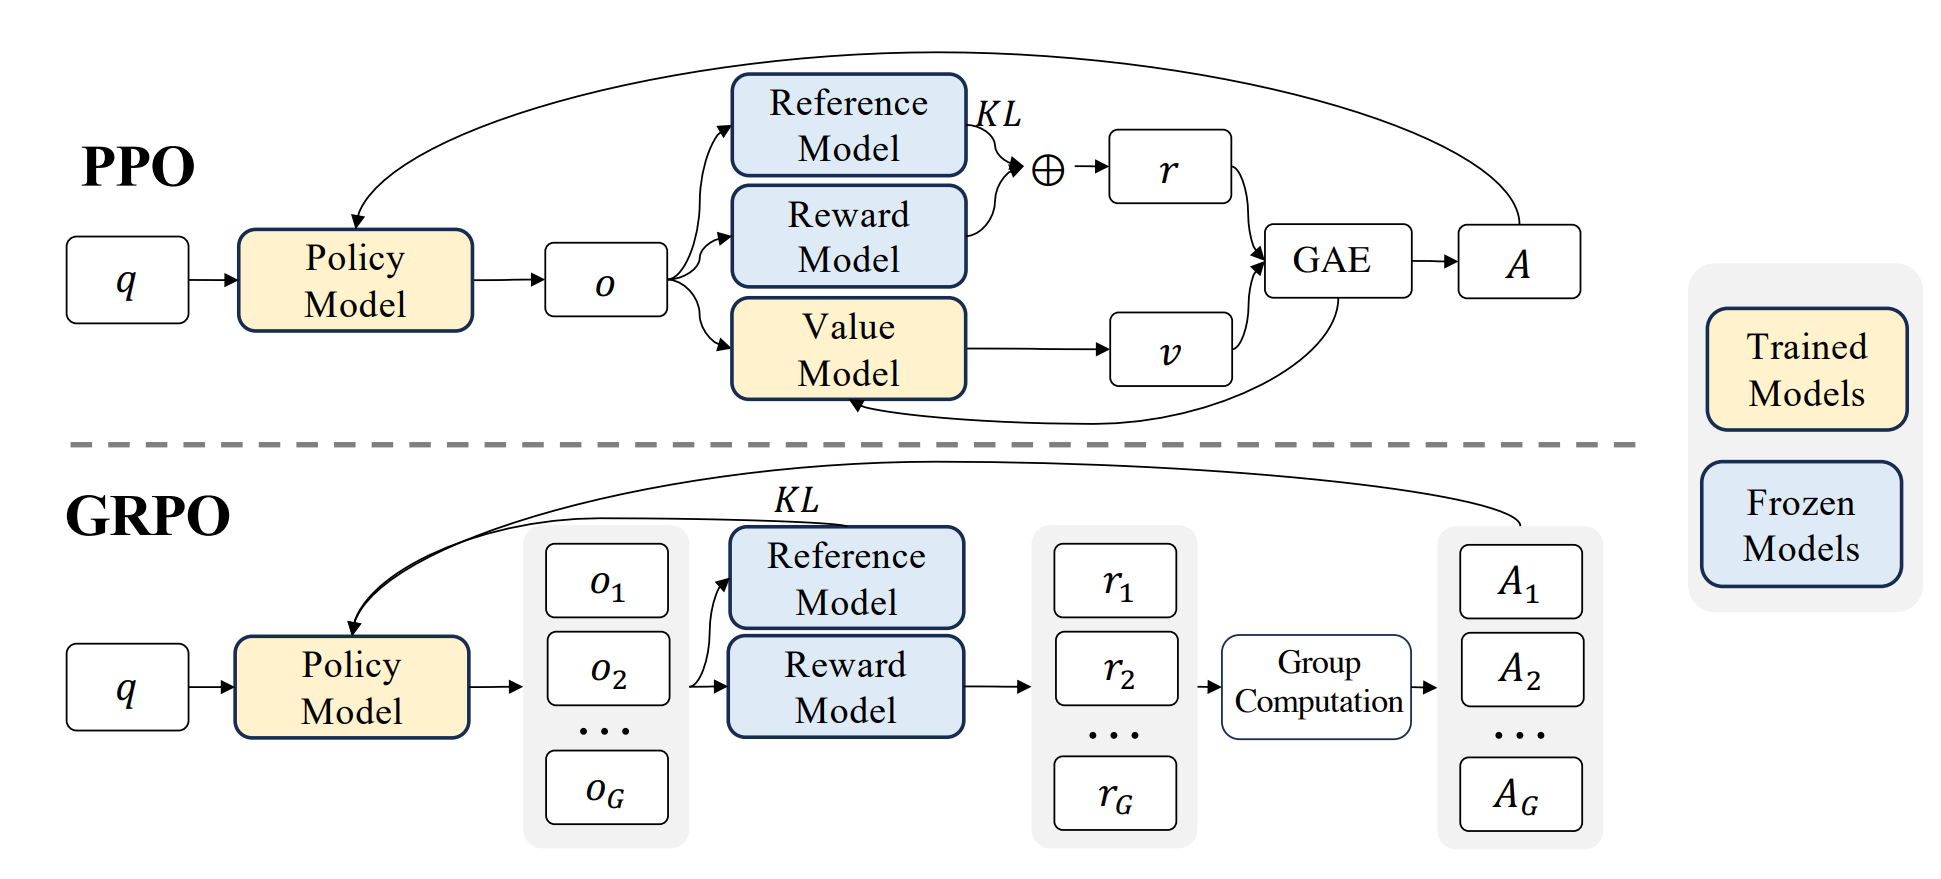
\includegraphics[width=\textwidth]{img/GRPO.png}
            \caption{GRPO算法框架}
        \end{figure}
    \end{columns}
\end{frame}

% 奖励函数设计
\begin{frame}{奖励函数设计}
    \begin{itemize}
        \item \textbf{准确性奖励(权重5)}
        \begin{itemize}
            \item $R_{accuracy} = \exp(-\text{MSE}(y_{pred}, y_{target}))$
            \item 预测数量影响:$R_{final} = R_{accuracy} \times \text{factor}$
            \item 位置误差分析
        \end{itemize}
        \vspace{0.2cm}
        \item \textbf{格式奖励(权重1)}
        \begin{itemize}
            \item 基本结构(0.4分):标签完整性
            \item 分析步骤(0.3分):推理过程
            \item 答案格式(0.3分):输出规范
        \end{itemize}
    \end{itemize}
\end{frame}

% 训练策略
\begin{frame}{训练策略}
    \begin{itemize}
        \item \textbf{模型配置}
        \begin{itemize}
            \item Qwen2.5-1.5B-Instruct模型
            \item 最大序列长度:800 tokens
            \item 温度系数:0.7,top-p:0.9
        \end{itemize}
        \vspace{0.2cm}
        \item \textbf{GRPO参数}
        \begin{itemize}
            \item $\beta$ 系数:0.04
            \item $\epsilon$ 阈值:0.2
            \item 每个输入生成4个候选结果
        \end{itemize}
    \end{itemize}
\end{frame}  % 项目背景与目标
\section{实验设计与结果}

% 训练过程分析
\begin{frame}{训练过程分析}
    \begin{columns}
        \column{0.5\textwidth}
        \begin{figure}
            \includegraphics[width=\textwidth]{img/accuracy_reward.png}
            \caption{准确性奖励变化}
        \end{figure}
        \column{0.5\textwidth}
        \begin{figure}
            \includegraphics[width=\textwidth]{img/format_reward.png}
            \caption{格式奖励变化}
        \end{figure}
    \end{columns}
    \begin{itemize}
        \item 准确性奖励:经过60轮训练后趋于稳定
        \item 格式奖励:快速收敛,保持高水平
    \end{itemize}
\end{frame}

% 模型对比分析
\begin{frame}{模型对比分析}
    \begin{columns}
        \column{0.5\textwidth}
        \begin{figure}
            \includegraphics[width=\textwidth]{img/mse_comparison_in_distribution.png}
            \caption{分布内MSE对比}
        \end{figure}
        \column{0.5\textwidth}
        \begin{figure}
            \includegraphics[width=\textwidth]{img/mse_comparison_out_of_distribution.png}
            \caption{分布外MSE对比}
        \end{figure}
    \end{columns}
    \begin{itemize}
        \item 1.5B模型在两个测试集上都显著优于0.5B模型
        \item 分布外测试集上的优势更为明显
    \end{itemize}
\end{frame}

% 位置误差分析
\begin{frame}{位置误差分析}
    \begin{columns}
        \column{0.5\textwidth}
        \begin{figure}
            \includegraphics[width=\textwidth]{img/position_errors_in_distribution.png}
            \caption{分布内位置误差}
        \end{figure}
        \column{0.5\textwidth}
        \begin{figure}
            \includegraphics[width=\textwidth]{img/position_errors_out_of_distribution.png}
            \caption{分布外位置误差}
        \end{figure}
    \end{columns}
    \begin{itemize}
        \item 1.5B模型误差增长更加平缓
        \item 表现出更强的预测稳定性
    \end{itemize}
\end{frame}

% 总结与展望
\begin{frame}{总结与展望}
    \begin{itemize}
        \item \textbf{主要创新点}
        \begin{itemize}
            \item 多维度奖励函数设计
            \item 详细的位置误差分析
            \item 分布内外泛化能力评估
        \end{itemize}
        \vspace{0.3cm}
        \item \textbf{未来工作}
        \begin{itemize}
            \item 扩展到更复杂的运动模式
            \item 优化奖励计算效率
            \item 提升模型泛化能力
        \end{itemize}
    \end{itemize}
\end{frame}

% 结束页
\begin{frame}
    \begin{center}
        \Huge 感谢聆听!
        \vspace{1cm}
        
        \Large Q \& A
    \end{center}
\end{frame}

% \begin{frame}{Referências}
%     \nocite{*}
%     \printbibliography[heading=none]
% \end{frame}  % 算法设计
% \section{实验设计与结果}

% 训练过程分析
\begin{frame}{训练过程分析}
    \begin{columns}
        \column{0.5\textwidth}
        \begin{figure}
            \includegraphics[width=\textwidth]{Images/accuracy_reward.png}
            \caption{准确性奖励变化}
        \end{figure}
        \column{0.5\textwidth}
        \begin{figure}
            \includegraphics[width=\textwidth]{Images/format_reward.png}
            \caption{格式奖励变化}
        \end{figure}
    \end{columns}
    \begin{itemize}
        \item 准确性奖励:经过60轮训练后趋于稳定
        \item 格式奖励:快速收敛,保持高水平
    \end{itemize}
\end{frame}

% 模型对比分析
\begin{frame}{模型对比分析}
    \begin{columns}
        \column{0.5\textwidth}
        \begin{figure}
            \includegraphics[width=\textwidth]{Images/mse_comparison_in_distribution.png}
            \caption{分布内MSE对比}
        \end{figure}
        \column{0.5\textwidth}
        \begin{figure}
            \includegraphics[width=\textwidth]{Images/mse_comparison_out_of_distribution.png}
            \caption{分布外MSE对比}
        \end{figure}
    \end{columns}
    \begin{itemize}
        \item 1.5B模型在两个测试集上都显著优于0.5B模型
        \item 分布外测试集上的优势更为明显
    \end{itemize}
\end{frame}

% 位置误差分析
\begin{frame}{位置误差分析}
    \begin{columns}
        \column{0.5\textwidth}
        \begin{figure}
            \includegraphics[width=\textwidth]{Images/position_errors_in_distribution.png}
            \caption{分布内位置误差}
        \end{figure}
        \column{0.5\textwidth}
        \begin{figure}
            \includegraphics[width=\textwidth]{Images/position_errors_out_of_distribution.png}
            \caption{分布外位置误差}
        \end{figure}
    \end{columns}
    \begin{itemize}
        \item 1.5B模型误差增长更加平缓
        \item 表现出更强的预测稳定性
    \end{itemize}
\end{frame}

% 总结与展望
\begin{frame}{总结与展望}
    \begin{itemize}
        \item \textbf{主要创新点}
        \begin{itemize}
            \item 多维度奖励函数设计
            \item 详细的位置误差分析
            \item 分布内外泛化能力评估
        \end{itemize}
        \vspace{0.3cm}
        \item \textbf{未来工作}
        \begin{itemize}
            \item 扩展到更复杂的运动模式
            \item 优化奖励计算效率
            \item 提升模型泛化能力
        \end{itemize}
    \end{itemize}
\end{frame}

% 结束页
\begin{frame}
    \begin{center}
        \Huge 感谢聆听!
        \vspace{1cm}
        
        \Large Q \& A
    \end{center}
\end{frame}

% \begin{frame}{Referências}
%     \nocite{*}
%     \printbibliography[heading=none]
% \end{frame}  % 实验设计与结果

% 结尾页
\begin{frame}
    \begin{center}
        {\Huge THANKS}
    \end{center}
\end{frame}

\end{document}
